%% bare_jrnl.tex
%% V1.4b
%% 2015/08/26
%% by Michael Shell
%% see http://www.michaelshell.org/
%% for current contact information.
%%
%% This is a skeleton file demonstrating the use of IEEEtran.cls
%% (requires IEEEtran.cls version 1.8b or later) with an IEEE
%% journal paper.
%%
%% Support sites:
%% http://www.michaelshell.org/tex/ieeetran/
%% http://www.ctan.org/pkg/ieeetran
%% and
%% http://www.ieee.org/

%%*************************************************************************
%% Legal Notice:
%% This code is offered as-is without any warranty either expressed or
%% implied; without even the implied warranty of MERCHANTABILITY or
%% FITNESS FOR A PARTICULAR PURPOSE! 
%% User assumes all risk.
%% In no event shall the IEEE or any contributor to this code be liable for
%% any damages or losses, including, but not limited to, incidental,
%% consequential, or any other damages, resulting from the use or misuse
%% of any information contained here.
%%
%% All comments are the opinions of their respective authors and are not
%% necessarily endorsed by the IEEE.
%%
%% This work is distributed under the LaTeX Project Public License (LPPL)
%% ( http://www.latex-project.org/ ) version 1.3, and may be freely used,
%% distributed and modified. A copy of the LPPL, version 1.3, is included
%% in the base LaTeX documentation of all distributions of LaTeX released
%% 2003/12/01 or later.
%% Retain all contribution notices and credits.
%% ** Modified files should be clearly indicated as such, including  **
%% ** renaming them and changing author support contact information. **
%%*************************************************************************


% *** Authors should verify (and, if needed, correct) their LaTeX system  ***
% *** with the testflow diagnostic prior to trusting their LaTeX platform ***
% *** with production work. The IEEE's font choices and paper sizes can   ***
% *** trigger bugs that do not appear when using other class files.       ***                          ***
% The testflow support page is at:
% http://www.michaelshell.org/tex/testflow/



\documentclass[journal]{IEEEtran}
%
% If IEEEtran.cls has not been installed into the LaTeX system files,
% manually specify the path to it like:
% \documentclass[journal]{../sty/IEEEtran}





% Some very useful LaTeX packages include:
% (uncomment the ones you want to load)


% *** MISC UTILITY PACKAGES ***
%
%\usepackage{ifpdf}
% Heiko Oberdiek's ifpdf.sty is very useful if you need conditional
% compilation based on whether the output is pdf or dvi.
% usage:
% \ifpdf
%   % pdf code
% \else
%   % dvi code
% \fi
% The latest version of ifpdf.sty can be obtained from:
% http://www.ctan.org/pkg/ifpdf
% Also, note that IEEEtran.cls V1.7 and later provides a builtin
% \ifCLASSINFOpdf conditional that works the same way.
% When switching from latex to pdflatex and vice-versa, the compiler may
% have to be run twice to clear warning/error messages.






% *** CITATION PACKAGES ***
%
%\usepackage{cite}
% cite.sty was written by Donald Arseneau
% V1.6 and later of IEEEtran pre-defines the format of the cite.sty package
% \cite{} output to follow that of the IEEE. Loading the cite package will
% result in citation numbers being automatically sorted and properly
% "compressed/ranged". e.g., [1], [9], [2], [7], [5], [6] without using
% cite.sty will become [1], [2], [5]--[7], [9] using cite.sty. cite.sty's
% \cite will automatically add leading space, if needed. Use cite.sty's
% noadjust option (cite.sty V3.8 and later) if you want to turn this off
% such as if a citation ever needs to be enclosed in parenthesis.
% cite.sty is already installed on most LaTeX systems. Be sure and use
% version 5.0 (2009-03-20) and later if using hyperref.sty.
% The latest version can be obtained at:
% http://www.ctan.org/pkg/cite
% The documentation is contained in the cite.sty file itself.


\usepackage{cite}
\usepackage{amsmath,amssymb,amsfonts}
\usepackage{algorithmic}
\usepackage{textcomp}
\usepackage{xcolor}
\usepackage{physics}


% *** GRAPHICS RELATED PACKAGES ***
%
\ifCLASSINFOpdf
  \usepackage[pdftex]{graphicx}
  % declare the path(s) where your graphic files are
  %\graphicspath{{../pdf/}{../jpeg/}{../png/}}
  % and their extensions so you won't have to specify these with
  % every instance of \includegraphics
   \DeclareGraphicsExtensions{.pdf,.png,.jpeg}
\else
  % or other class option (dvipsone, dvipdf, if not using dvips). graphicx
  % will default to the driver specified in the system graphics.cfg if no
  % driver is specified.
   \usepackage[dvips]{graphicx}
  % declare the path(s) where your graphic files are
  % \graphicspath{{../eps/}}
  % and their extensions so you won't have to specify these with
  % every instance of \includegraphics
  % \DeclareGraphicsExtensions{.eps}
\fi
% graphicx was written by David Carlisle and Sebastian Rahtz. It is
% required if you want graphics, photos, etc. graphicx.sty is already
% installed on most LaTeX systems. The latest version and documentation
% can be obtained at: 
% http://www.ctan.org/pkg/graphicx
% Another good source of documentation is "Using Imported Graphics in
% LaTeX2e" by Keith Reckdahl which can be found at:
% http://www.ctan.org/pkg/epslatex
%
% latex, and pdflatex in dvi mode, support graphics in encapsulated
% postscript (.eps) format. pdflatex in pdf mode supports graphics
% in .pdf, .jpeg, .png and .mps (metapost) formats. Users should ensure
% that all non-photo figures use a vector format (.eps, .pdf, .mps) and
% not a bitmapped formats (.jpeg, .png). The IEEE frowns on bitmapped formats
% which can result in "jaggedy"/blurry rendering of lines and letters as
% well as large increases in file sizes.
%
% You can find documentation about the pdfTeX application at:
% http://www.tug.org/applications/pdftex





% *** MATH PACKAGES ***
%
%\usepackage{amsmath}
% A popular package from the American Mathematical Society that provides
% many useful and powerful commands for dealing with mathematics.
%
% Note that the amsmath package sets \interdisplaylinepenalty to 10000
% thus preventing page breaks from occurring within multiline equations. Use:
%\interdisplaylinepenalty=2500
% after loading amsmath to restore such page breaks as IEEEtran.cls normally
% does. amsmath.sty is already installed on most LaTeX systems. The latest
% version and documentation can be obtained at:
% http://www.ctan.org/pkg/amsmath


 


% *** SPECIALIZED LIST PACKAGES ***
%
%\usepackage{algorithmic}
% algorithmic.sty was written by Peter Williams and Rogerio Brito.
% This package provides an algorithmic environment fo describing algorithms.
% You can use the algorithmic environment in-text or within a figure
% environment to provide for a floating algorithm. Do NOT use the algorithm
% floating environment provided by algorithm.sty (by the same authors) or
% algorithm2e.sty (by Christophe Fiorio) as the IEEE does not use dedicated
% algorithm float types and packages that provide these will not provide
% correct IEEE style captions. The latest version and documentation of
% algorithmic.sty can be obtained at:
% http://www.ctan.org/pkg/algorithms
% Also of interest may be the (relatively newer and more customizable)
% algorithmicx.sty package by Szasz Janos:
% http://www.ctan.org/pkg/algorithmicx




% *** ALIGNMENT PACKAGES ***
%
%\usepackage{array}
% Frank Mittelbach's and David Carlisle's array.sty patches and improves
% the standard LaTeX2e array and tabular environments to provide better
% appearance and additional user controls. As the default LaTeX2e table
% generation code is lacking to the point of almost being broken with
% respect to the quality of the end results, all users are strongly
% advised to use an enhanced (at the very least that provided by array.sty)
% set of table tools. array.sty is already installed on most systems. The
% latest version and documentation can be obtained at:
% http://www.ctan.org/pkg/array


% IEEEtran contains the IEEEeqnarray family of commands that can be used to
% generate multiline equations as well as matrices, tables, etc., of high
% quality.




% *** SUBFIGURE PACKAGES ***
%\ifCLASSOPTIONcompsoc
%  \usepackage[caption=false,font=normalsize,labelfont=sf,textfont=sf]{subfig}
%\else
%  \usepackage[caption=false,font=footnotesize]{subfig}
%\fi
% subfig.sty, written by Steven Douglas Cochran, is the modern replacement
% for subfigure.sty, the latter of which is no longer maintained and is
% incompatible with some LaTeX packages including fixltx2e. However,
% subfig.sty requires and automatically loads Axel Sommerfeldt's caption.sty
% which will override IEEEtran.cls' handling of captions and this will result
% in non-IEEE style figure/table captions. To prevent this problem, be sure
% and invoke subfig.sty's "caption=false" package option (available since
% subfig.sty version 1.3, 2005/06/28) as this is will preserve IEEEtran.cls
% handling of captions.
% Note that the Computer Society format requires a larger sans serif font
% than the serif footnote size font used in traditional IEEE formatting
% and thus the need to invoke different subfig.sty package options depending
% on whether compsoc mode has been enabled.
%
% The latest version and documentation of subfig.sty can be obtained at:
% http://www.ctan.org/pkg/subfig




% *** FLOAT PACKAGES ***
%
%\usepackage{fixltx2e}
% fixltx2e, the successor to the earlier fix2col.sty, was written by
% Frank Mittelbach and David Carlisle. This package corrects a few problems
% in the LaTeX2e kernel, the most notable of which is that in current
% LaTeX2e releases, the ordering of single and double column floats is not
% guaranteed to be preserved. Thus, an unpatched LaTeX2e can allow a
% single column figure to be placed prior to an earlier double column
% figure.
% Be aware that LaTeX2e kernels dated 2015 and later have fixltx2e.sty's
% corrections already built into the system in which case a warning will
% be issued if an attempt is made to load fixltx2e.sty as it is no longer
% needed.
% The latest version and documentation can be found at:
% http://www.ctan.org/pkg/fixltx2e


%\usepackage{stfloats}
% stfloats.sty was written by Sigitas Tolusis. This package gives LaTeX2e
% the ability to do double column floats at the bottom of the page as well
% as the top. (e.g., "\begin{figure*}[!b]" is not normally possible in
% LaTeX2e). It also provides a command:
%\fnbelowfloat
% to enable the placement of footnotes below bottom floats (the standard
% LaTeX2e kernel puts them above bottom floats). This is an invasive package
% which rewrites many portions of the LaTeX2e float routines. It may not work
% with other packages that modify the LaTeX2e float routines. The latest
% version and documentation can be obtained at:
% http://www.ctan.org/pkg/stfloats
% Do not use the stfloats baselinefloat ability as the IEEE does not allow
% \baselineskip to stretch. Authors submitting work to the IEEE should note
% that the IEEE rarely uses double column equations and that authors should try
% to avoid such use. Do not be tempted to use the cuted.sty or midfloat.sty
% packages (also by Sigitas Tolusis) as the IEEE does not format its papers in
% such ways.
% Do not attempt to use stfloats with fixltx2e as they are incompatible.
% Instead, use Morten Hogholm'a dblfloatfix which combines the features
% of both fixltx2e and stfloats:
%
% \usepackage{dblfloatfix}
% The latest version can be found at:
% http://www.ctan.org/pkg/dblfloatfix

\usepackage{url}


%\ifCLASSOPTIONcaptionsoff
%  \usepackage[nomarkers]{endfloat}
% \let\MYoriglatexcaption\caption
% \renewcommand{\caption}[2][\relax]{\MYoriglatexcaption[#2]{#2}}
%\fi
% endfloat.sty was written by James Darrell McCauley, Jeff Goldberg and 
% Axel Sommerfeldt. This package may be useful when used in conjunction with 
% IEEEtran.cls'  captionsoff option. Some IEEE journals/societies require that
% submissions have lists of figures/tables at the end of the paper and that
% figures/tables without any captions are placed on a page by themselves at
% the end of the document. If needed, the draftcls IEEEtran class option or
% \CLASSINPUTbaselinestretch interface can be used to increase the line
% spacing as well. Be sure and use the nomarkers option of endfloat to
% prevent endfloat from "marking" where the figures would have been placed
% in the text. The two hack lines of code above are a slight modification of
% that suggested by in the endfloat docs (section 8.4.1) to ensure that
% the full captions always appear in the list of figures/tables - even if
% the user used the short optional argument of \caption[]{}.
% IEEE papers do not typically make use of \caption[]'s optional argument,
% so this should not be an issue. A similar trick can be used to disable
% captions of packages such as subfig.sty that lack options to turn off
% the subcaptions:
% For subfig.sty:
% \let\MYorigsubfloat\subfloat
% \renewcommand{\subfloat}[2][\relax]{\MYorigsubfloat[]{#2}}
% However, the above trick will not work if both optional arguments of
% the \subfloat command are used. Furthermore, there needs to be a
% description of each subfigure *somewhere* and endfloat does not add
% subfigure captions to its list of figures. Thus, the best approach is to
% avoid the use of subfigure captions (many IEEE journals avoid them anyway)
% and instead reference/explain all the subfigures within the main caption.
% The latest version of endfloat.sty and its documentation can obtained at:
% http://www.ctan.org/pkg/endfloat
%
% The IEEEtran \ifCLASSOPTIONcaptionsoff conditional can also be used
% later in the document, say, to conditionally put the References on a 
% page by themselves.




% *** PDF, URL AND HYPERLINK PACKAGES ***
%
%\usepackage{url}
% url.sty was written by Donald Arseneau. It provides better support for
% handling and breaking URLs. url.sty is already installed on most LaTeX
% systems. The latest version and documentation can be obtained at:
% http://www.ctan.org/pkg/url
% Basically, \url{my_url_here}.




% *** Do not adjust lengths that control margins, column widths, etc. ***
% *** Do not use packages that alter fonts (such as pslatex).         ***
% There should be no need to do such things with IEEEtran.cls V1.6 and later.
% (Unless specifically asked to do so by the journal or conference you plan
% to submit to, of course. )


% correct bad hyphenation here
\hyphenation{op-tical net-works semi-conduc-tor}


\begin{document}
%
% paper title
% Titles are generally capitalized except for words such as a, an, and, as,
% at, but, by, for, in, nor, of, on, or, the, to and up, which are usually
% not capitalized unless they are the first or last word of the title.
% Linebreaks \\ can be used within to get better formatting as desired.
% Do not put math or special symbols in the title.
\title{Robotic Perception and Action Project Report \\EMG Classification using deep learning}
%
%
% author names and IEEE memberships
% note positions of commas and nonbreaking spaces ( ~ ) LaTeX will not break
% a structure at a ~ so this keeps an author's name from being broken across
% two lines.
% use \thanks{} to gain access to the first footnote area
% a separate \thanks must be used for each paragraph as LaTeX2e's \thanks
% was not built to handle multiple paragraphs
%

\author{Riccardo~Ballaben,~\IEEEmembership{211784,} \\ %\ldots  ,
Giorgio~Checola,~\IEEEmembership{215475,}  \\
Meron~Hailu, ~\IEEEmembership{214146}
        }% <-this % stops a space



% note the % following the last \IEEEmembership and also \thanks - 
% these prevent an unwanted space from occurring between the last author name
% and the end of the author line. i.e., if you had this:
% 
% \author{....lastname \thanks{...} \thanks{...} }
%                     ^------------^------------^----Do not want these spaces!
%
% a space would be appended to the last name and could cause every name on that
% line to be shifted left slightly. This is one of those "LaTeX things". For
% instance, "\textbf{A} \textbf{B}" will typeset as "A B" not "AB". To get
% "AB" then you have to do: "\textbf{A}\textbf{B}"
% \thanks is no different in this regard, so shield the last } of each \thanks
% that ends a line with a % and do not let a space in before the next \thanks.
% Spaces after \IEEEmembership other than the last one are OK (and needed) as
% you are supposed to have spaces between the names. For what it is worth,
% this is a minor point as most people would not even notice if the said evil
% space somehow managed to creep in.


% The paper headers
%\markboth{Journal of \LaTeX\ Class Files,~Vol.~14, No.~8, August~2015}%
%{Shell \MakeLowercase{\textit{et al.}}: Bare Demo of IEEEtran.cls for IEEE Journals}
% The only time the second header will appear is for the odd numbered pages
% after the title page when using the twoside option.
% 
% *** Note that you probably will NOT want to include the author's ***
% *** name in the headers of peer review papers.                   ***
% You can use \ifCLASSOPTIONpeerreview for conditional compilation here if
% you desire.




% If you want to put a publisher's ID mark on the page you can do it like
% this:
%\IEEEpubid{0000--0000/00\$00.00~\copyright~2015 IEEE}
% Remember, if you use this you must call \IEEEpubidadjcol in the second
% column for its text to clear the IEEEpubid mark.



% use for special paper notices
%\IEEEspecialpapernotice{(Invited Paper)}




% make the title area
\maketitle

% As a general rule, do not put math, special symbols or citations
% in the abstract or keywords.
\begin{abstract}
This report summaries the content of the work.\\
The project consisted in classifying a a dataset of EMG signal of a ....with respect to a class of movements, by means of machine learning algorithms taught in class.  \\
We have managed to reach an accuracy of 85\%
%The abstract goes here.
%The abstract should resume your report in few sentences. \\
%1) Surround the context;\\
%2) Motivate the goal of the work;\\
%3) Anticipate the most important results or achievements.\\
%200 words maximum

\end{abstract}

% Note that keywords are not normally used for peerreview papers.
%\begin{IEEEkeywords}
%IEEE, IEEEtran, journal, \LaTeX, paper, template.
%\end{IEEEkeywords}






% For peer review papers, you can put extra information on the cover
% page as needed:
% \ifCLASSOPTIONpeerreview
% \begin{center} \bfseries EDICS Category: 3-BBND \end{center}
% \fi
%
% For peerreview papers, this IEEEtran command inserts a page break and
% creates the second title. It will be ignored for other modes.
\IEEEpeerreviewmaketitle



\section{Introduction}
% The very first letter is a 2 line initial drop letter followed
% by the rest of the first word in caps.
% 
% form to use if the first word consists of a single letter:
% \IEEEPARstart{A}{demo} file is ....
% 
% form to use if you need the single drop letter followed by
% normal text (unknown if ever used by the IEEE):
% \IEEEPARstart{A}{}demo file is ....
% 
% Some journals put the first two words in caps:
% \IEEEPARstart{T}{his demo} file is ....
% 
% Here we have the typical use of a "T" for an initial drop letter
% and "HIS" in caps to complete the first word.
\IEEEPARstart{T}{his} demo file is intended to serve as a ``starter file''.
The template can be found here~\cite{IEEEexample:IEEEtemplate}:\\ \url{http://www.ieee.org/conferences_events/conferences/publishing/templates.html }\\
\\
\\
\\
The study on the specific field, thanks to the progress in technology has increased a lot in the last year also thanks to the progress of the Artificial Intelligence. The possibility to study and analyse the signal obtained from a certain gesture could make big progress for the sake of amputees if then applied at the robotic arm technology.


By using the software MATLAB we analyzed a dataset of EMG using machine learning techniques explained in class. 
\\
signals elaborating a spesific LSTM structure in order to reach the highest accuracy as possibile. 
We did a comparison using two kind of supervised learning analysis, that are LSTM using the signal and DNN usign the features extracted from the signal.
%The introduction should take 3 columns and the main purposes are: 
%\begin{itemize}
%    \item Describe the problem;
%    \item State the contributions of the project work.
%\end{itemize}

%The best way to tell the story is to organize the introduction in 4 parts: 
%\begin{enumerate}
%    \item Introduce the context of the work (e.g., internet of things, artificial intelligence, industrial electronics, smart grids, \ldots). Describe also the possible scenarios where the project can be used. Then highlight the open challenges or issues and problems to be solved ($\approx ~one~column$);
%    \item Describe possible solutions, new technologies, or recent innovations that can fill the gap and solve the open challenges. You can cite some recent papers, scientific articles about such technologies. Then, start to describe the work done and the project objectives ($\approx ~one~column$);
%    \item State the contribution of the project. The list of contributions drives the entire report: the rest of the pages substantiate the claims you make here. 
%    Use bullet list for the contributions ($\approx half~a~column$);
%    \item Describe the organization of the report. (e.g.,
%    \textit{ \ldots The rest of the report  is organized as follows. Related Work is reviewed in Section~II. Section~III presents the technology used; we describe the hardware and software developed in the project. \ldots Section~X describes simulation and experimental results compared to state-of-art. Section~N concludes the report.}) ($\approx half~a~column$).
%\end{enumerate}

% You must have at least 2 lines in the paragraph with the drop letter
% (should never be an issue)

\section{Related Work}
%This section is necessary and should take about 1,5 column. 
%\\
%Please take the time to read and report some scientific papers related to the activities done in the projects. Try to describe what the authors of the papers did, what they achieved. Then try to compare their work to your project. What is different? 
%Do you outperform some of the articles you find?  Did you demonstrate it?   
%A state of the art of 4-5 papers is enough.
%\\
%\\
%Literature search can be started using the following libraries: IEEExplore, Google Scholar, ACM digital libray. \\
%- \url{https://ieeexplore.ieee.org/Xplore/home.jsp}\\
%- \url{https://scholar.google.it}\\
%- \url{https://dl.acm.org}\\
%\\
%Some library needs a subscription. The university provides access to the most important digital library. Connecting from the UNITN intranet network permits you to browse and download documents with no problems. If you are out of the UNITN intranet, you need a VPN. Information about the university VPN-OUT can be found here: \\  
%\\
%- \url{https://icts.unitn.it/case/it/catalog/vpnout/}\\
%- \url{https://wiki.unitn.it/pub:conf-vpn-out}\\
%\\
%You may start a literature search from some Keywords related your project work. 
%Then, we you find something relevant, you may use several strategies: 
%\begin{itemize}
%    \item Focus on the authors. If the authors work on a specific topic, they probably have published other research results in the same field. (Search based on authors).
%    \item Focus on previous works. The last part of a scientific paper contains the bibliography. The references link to previously published papers, that the authors consider essential to understanding their manuscript. They deserve a brief overlook at least, and likely you may find useful information on the topic (Back to the past)
%    \item Focus on who cited the paper. All the digital libraries (e.g., IEEE, Google Scholar, \ldots) provide a metric about how many later-articles, have cited the paper. If the paper is quite recent, and yet collected a quite high number of citation, maybe it is worth to open it and check (Jump to the \textsl{future}). 
%\end{itemize}.
%\\
%Please, consider that the ICT innovation paces very fast. Apart from few cornerstones,  papers of 5-years ago probably contain already outdated information and technology. Thus prefer focusing on articles no earlier than 3-4 years ago..


\section{Elaborating the project}
%\section{Description of the work for the project}
We took a dataset of rami khushaba. It is composed by EMG signal of 8 subjects, six males and two females, aged between 20-35 years were recruited to perform the required fingers movements. The subjects were all normally limbed with no neurological or muscular disorders. 

The datasets were recorded using eight EMG channels (DE 2.x series EMG sensors) mounted across the circumference of the forearm and processed by the Bagnoli desktop EMG system from Delsys Inc., as shown in Fig.2. A 2-slot adhesive skin interface was applied on each of the sensors to firmly stick them to the skin. A conductive adhesive reference electrode, dermatrode reference electrode, was placed on the wrist of each of the subjects during the experiments. The collected EMG signals were amplified using a Delsys Bagnoli-8 amplifier to a total gain of 1000. A 12-bit analog-to-digital converter (National Instruments, BNC-2090) was used to sample the signal at 4000 Hz; the signal data were then acquired using Delsys EMGWorks Acquisition software. The EMG signals were then bandpass filtered between 20-450 Hz with a notch filter implemented to remove the 50 Hz line interference. Fifteen classes of movements were collected during this experiment including: the flexion of each of the individual fingers, i.e., Thumb (T), Index (I), Middle (M), Ring (R), Little (L) and the combined Thumb-Index (T-I), Thumb-Middle (T-M), Thumb-Ring (T-R), Thumb-Little (TL), Index-Middle (I-M), Middle-Ring (M-R), Ring-Little (RL), Index-Middle-Ring (I-M-R), Middle-Ring-Little (M-RL), and finally the hand close class (HC) as shown in Fig.3. 

*** When collecting data, the subjects were asked to perform each of the aforementioned fifteen movements, and hold that movement for a period of 20 seconds in each trial (only first 5 sec from each trial used in the paper). You can study what happened to the muscle, in terms of fatigue on this data, or do classification on it. Three trials are available (6 used in the paper, 3 provided here), allocate two of them for training and one for testing. You can even chop the extra data if you think 5 seconds are more than enough for each trial.

\begin{figure}[h]
	\centering{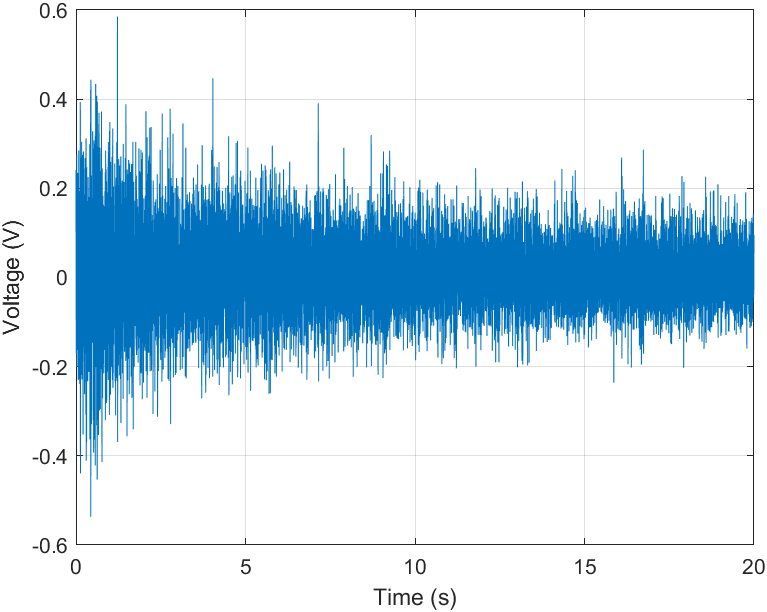
\includegraphics[width=50mm]{images/plot1}}
	\caption{Example of a figure caption.}
	\label{fig1}
\end{figure}

We did a preprocessing of the signal starting from filtering it. To do that we started plotting the fft to see it if the filter was necessary: we Compute two sided spectrum, Divide by L for normalisation of the power of the output for the length of the input signal and Compute signal sided spectrum by taking the positive part of double

\begin{figure}[h]
	\centering{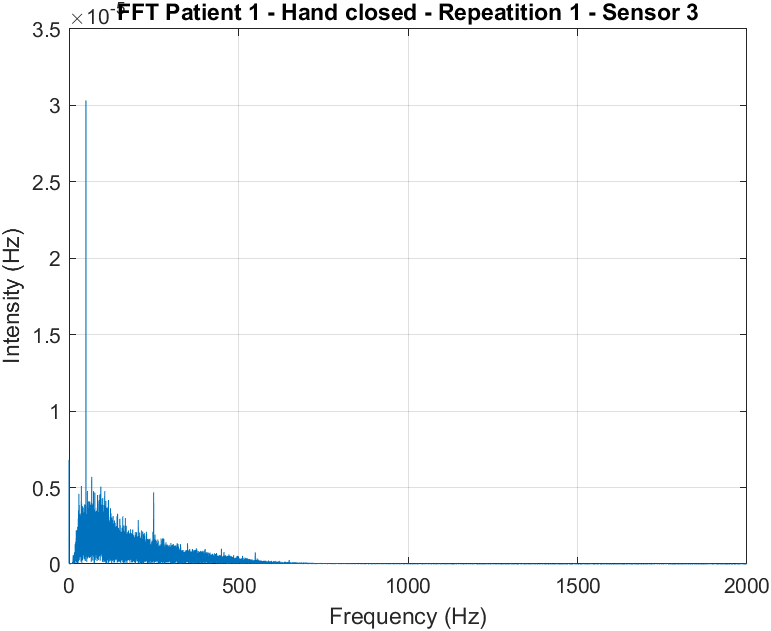
\includegraphics[width=50mm]{images/fft1}}
	\caption{Example of a figure caption.}
	\label{fig2}
\end{figure}
As you can see the signal was not filtered. So we did it applying a forth order Butterworth bandpass filter between 20 and 450 Hz and a notch filter at 50 Hz (more precisely from 48 to 52 Hz).
You can see from the pictures below the differences from the raw signal to the one filtered
\begin{figure}[h]
	\centering{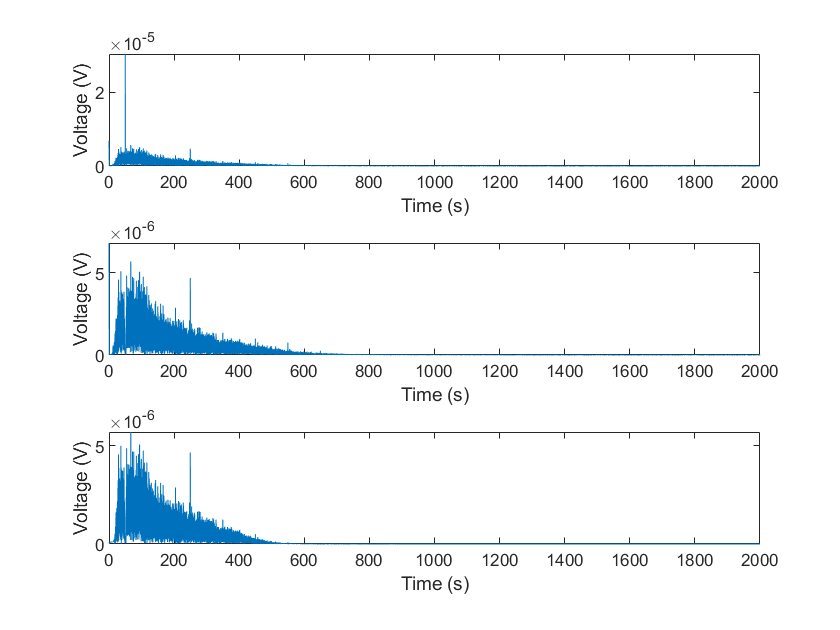
\includegraphics[width=70mm]{images/comparison1}}
	\caption{Example of a figure caption.}
	\label{fig3}
\end{figure}

Backing to time domain, the signal conditioning was not finished: we rectified it taking the absolute value
\begin{figure}[h]
	\centering{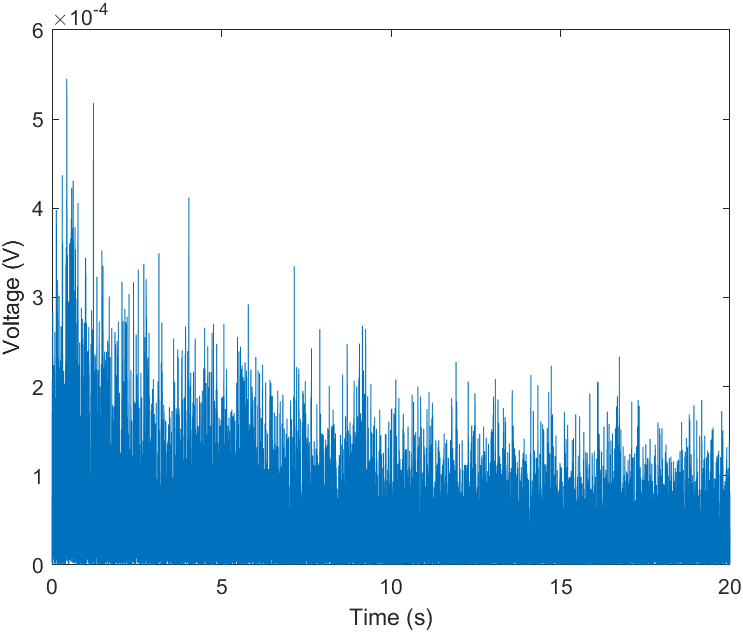
\includegraphics[width=50mm]{images/rectified1}}
	\caption{Example of a figure caption.}
	\label{fig4}
\end{figure}
And normalized between 0 and 1:
\begin{figure}[h]
	\centering{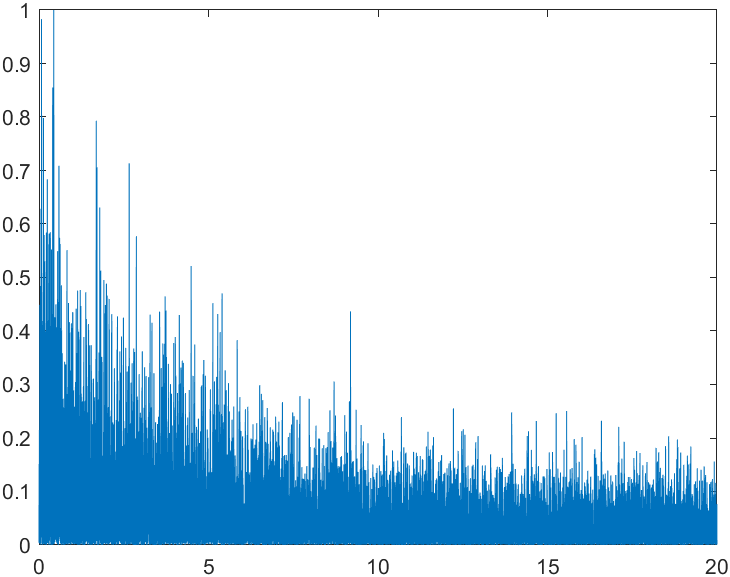
\includegraphics[width=50mm]{images/normalized1}}
	\caption{Example of a figure caption.}
	\label{fig5}
\end{figure}
Now we are ready for the implementation with LSTM.

CITAZIONI:
Even though the time consumption and dimension for TD features were
faster and smaller than other features, recognition performance was not satisfactory as claimed by
Tsai et al. [29].
\\
normalization
is a crucial step and changes in EMG amplitude can influence the normalization result, affecting
recognition performance.
\\


\subsection{LSTM}
For the labeling we gave a number at each movement converting the xls file into a number taking care that each movement had a different value. In this way we were not worried about assigning other type of label and something like that.

We feed the network with a cell array of $N\text{x}1$ cells, which include matrices of $8\text{x}100$ value. N is the total number of segments given to the network. We decided to split the signal in small segment of 0.5 sec in order to make easier the work for the neural network and increasing the final accuracy. \\
The 8 rows of the matrix represent the input of the network, the 8 sensor channel attached to the subjects, from which we got the EMG signals, while 100 columns are the value we took from each window, using a function to got the 100 bigger values. 
\subsection{Feature extraction}
Besides the analysis with LSTM we followed another method, more classic, consisting on extracting manually a set of features from the signals, giving them as inputs to a neural network in order to reach the same goal of the previous study.


There exist three types of EMG features: time-domain (TD), frequency-domain (FD) and time-frequency-domain (TFD) features. \\ 
Angkoon Phinyomark et al said that EMG features based on frequency-domain are not good in EMG signal classification. Moreover we discovered that many features are redundant, and their power changes depending also on the type of classifier you use for the process.
\\
In the end we opted for the ones that Angkoon Phinyomark et al considered the recommendation for each group in which features can be divided:
\begin{itemize}
	\item MAV from energy information method
	\item WL from complexity information method
	\item WAMP from frequency information method
	\item AR from prediction model method
	\item MAVSLP from time-dependence method
\end{itemize}

\begin{enumerate}
	\item Mean absolute value (MAV):
	\begin{equation}
	\text{MAV} = \frac{1}{N}\sum_{n=1}^{N}\abs{x_i}
	\label{eq1}
	\end{equation}
	
	\item Waveform length (WL):
	\begin{equation}
	\text{WL} = \sum_{n=1}^{N-1}\abs{x_{i+1}-x_i}
	\label{eq2}
	\end{equation}
	
	\item Willison amplitude (WAMP):
	\begin{equation}
	\text{WAMP} =\sum_{n=1}^{N-1}[f(\abs{x_n-x_{n+1}})]
	\label{eq3}
	\end{equation}
	
	where $f(x)= \begin{cases}
	1,	& \text{if } x\geq \text{threshold} \\
	0,  & \text{otherwise}
	\end{cases}$
	
	\item Auto-regressive coefficients (AR):
	\begin{equation}
	x_i=\frac{1}{N}\sum_{p=1}^{P}a_px_{i-p}+w_i
	\label{eq4}
	\end{equation}
	
	\item Mean absolute value slope (MAVSLP):
	\begin{equation}
	\text{MAVSLP}_k= \text{MAV}_{k+1}-\text{MAV}_k, \quad k = 1,...,K-1
	\label{eq5}
	\end{equation}
\end{enumerate}
We also add RMS since appears to be the best parameter compared to MAV, MAX, SSC, ZC and WL as it provides a quantitative measure for electrode selection \cite{b3}.
\begin{equation}
\text{RMS}= \sqrt{\frac{1}{N}\sum_{i=1}^{N}x_i^2}
\label{eq5}
\end{equation}

Feature in time domain do not need any transformation, which calculate based on raw EMG time series \cite{b3}.
For this reason we used the raw signal, only filtered with Notch at 50 Hz and band-pass between 20 and 450 Hz.

\subsection{DNN}
Once extracted the features we feed the network writing a MATLAB function that returns a vector with all the features. A vector for each segment in which we divided the 20 sec sequence. Choosing 0.5 sec, we got 40 segments. 

\section{Experimental results}
Add a Section about experimental results and verification of your output. 

Any number, both final and intermediate results should be described. Even the experimental setup, and the measurement environment should be described. The measure should be reproducible by the readers. Listing the models of the instrument is not important (e.g.,  oscilloscope TD98445.... ), while the type of instrumentation or the type of measure is fundamental to repeat the experiment. \\
\\
In case, please, provide a shared folder (e.g., github, gitlab, Google Drive, ... ) where the code is available for repeat the experiments, the achieved results are available for a comparison. 



\section{Conclusion}
sdasdadasdasd
\\
Context/Scenario  $\Rightarrow$  Challenges  $\Rightarrow$\\
 $\Rightarrow$ What you have done $\Rightarrow$ \\
 $\Rightarrow$ most important achievements, with key numbers. 
\\

\begin{thebibliography}{00}
	\bibitem{b1} R. N. Khushaba and Sarath Kodagoda, ``Electromyogram (EMG) Feature Reduction Using Mutual Components Analysis for Multifunction Prosthetic Fingers Control'', in Proc. Int. Conf. on Control, Automation, Robotics \& Vision (ICARCV), Guangzhou, 2012, pp. 1534-1539. (6 pages)
	\bibitem{b2} A. Phinyomark, P. Phukpattaranont, C. Limsakul, ``Feature reduction and selection for EMG signal classification'', 3rd ed., vol. 2. Oxford: Clarendon, 1892, pp.68--73.
	\bibitem{b3} Kendell, C.; Lemaire, E.D.; Losier, Y.; Chan, A.; Hudgins, B. A novel approach to surface electromyography:
	An exploratory study of electrode-pair selection based on signal characteristics. J. Neuro Eng. Rehabil. 2012,
	9, doi:10.1186/1743-0003-9-24.
	\bibitem{b4} K. Elissa, ``Title of paper if known,'' unpublished.
	\bibitem{b5} R. Nicole, ``Title of paper with only first word capitalized,'' J. Name Stand. Abbrev., in press.
	\bibitem{b6} Y. Yorozu, M. Hirano, K. Oka, and Y. Tagawa, ``Electron spectroscopy studies on magneto-optical media and plastic substrate interface,'' IEEE Transl. J. Magn. Japan, vol. 2, pp. 740--741, August 1987 [Digests 9th Annual Conf. Magnetics Japan, p. 301, 1982].
	\bibitem{b7} M. Young, The Technical Writer's Handbook. Mill Valley, CA: University Science, 1989.
\end{thebibliography}

% if have a single appendix:
%\appendix[Proof of the Zonklar Equations]
% or
%\appendix  % for no appendix heading
% do not use \section anymore after \appendix, only \section*
% is possibly needed

% use appendices with more than one appendix
% then use \section to start each appendix
% you must declare a \section before using any
% \subsection or using \label (\appendices by itself
% starts a section numbered zero.)
%


% \appendices
% \section{Proof of the First Zonklar Equation}
% Appendix one text goes here.

% % you can choose not to have a title for an appendix
% % if you want by leaving the argument blank
% \section{}
% Appendix two text goes here.


% % use section* for acknowledgment
% \section*{Acknowledgment}


% The authors would like to thank...


% Can use something like this to put references on a page
% by themselves when using endfloat and the captionsoff option.
\ifCLASSOPTIONcaptionsoff
  \newpage
\fi



% trigger a \newpage just before the given reference
% number - used to balance the columns on the last page
% adjust value as needed - may need to be readjusted if
% the document is modified later
%\IEEEtriggeratref{8}
% The "triggered" command can be changed if desired:
%\IEEEtriggercmd{\enlargethispage{-5in}}

% references section

% can use a bibliography generated by BibTeX as a .bbl file
% BibTeX documentation can be easily obtained at:
% http://mirror.ctan.org/biblio/bibtex/contrib/doc/
% The IEEEtran BibTeX style support page is at:
% http://www.michaelshell.org/tex/ieeetran/bibtex/
%\bibliographystyle{IEEEtran}
% argument is your BibTeX string definitions and bibliography database(s)
%\bibliography{IEEEabrv,../bib/paper}
%
% <OR> manually copy in the resultant .bbl file
% set second argument of \begin to the number of references
% % (used to reserve space for the reference number labels box)
% \begin{thebibliography}{1}

% \bibitem{IEEEhowto:kopka}
% H.~Kopka and P.~W. Daly, \emph{A Guide to \LaTeX}, 3rd~ed.\hskip 1em plus
%   0.5em minus 0.4em\relax Harlow, England: Addison-Wesley, 1999.

% \end{thebibliography}

\bibliographystyle{./IEEEtran}
\bibliography{./IEEEabrv,./IEEEexample}



% biography section
% 
% If you have an EPS/PDF photo (graphicx package needed) extra braces are
% needed around the contents of the optional argument to biography to prevent
% the LaTeX parser from getting confused when it sees the complicated
% \includegraphics command within an optional argument. (You could create
% your own custom macro containing the \includegraphics command to make things
% simpler here.)
%\begin{IEEEbiography}[{\includegraphics[width=1in,height=1.25in,clip,keepaspectratio]{mshell}}]{Michael Shell}
% or if you just want to reserve a space for a photo:

% \begin{IEEEbiography}{Michael Shell}
% Biography text here.
% \end{IEEEbiography}

% % if you will not have a photo at all:
% \begin{IEEEbiographynophoto}{John Doe}
% Biography text here.
% \end{IEEEbiographynophoto}

% % insert where needed to balance the two columns on the last page with
% % biographies
% %\newpage

% \begin{IEEEbiographynophoto}{Jane Doe}
% Biography text here.
% \end{IEEEbiographynophoto}

% % You can push biographies down or up by placing
% % a \vfill before or after them. The appropriate
% % use of \vfill depends on what kind of text is
% on the last page and whether or not the columns
% are being equalized.

%\vfill

% Can be used to pull up biographies so that the bottom of the last one
% is flush with the other column.
%\enlargethispage{-5in}



% that's all folks
\end{document}


